\section{Pre/Post Processing}
During our initial experiments, we observed a significant drop in training convergence speed when applying our WZ quantization.
We propose 2 design choices to rectify this and investigate their effectiveness: (i) per-layer normalization (e.g., 99th-percentile scaling) keeps dynamic ranges comparable across layers and rounds; and (ii) more active outlier handling to reduce the impact of extreme values on training.

\subsection{Normalization and Per-Layer Distribution}
If we consider the layer-by-layer nature of feedforward neural networks, we can intuitively assume that any distortion introduced in one layer will be propagated and potentially amplified in subsequent layers. This distortion should be considered as relative to the weights of that layer and not the entire model, as each layer has its own distribution of weights and gradients.
Now if we look at the distribution of weights per layer, as in Figure~\ref{fig:custom_cnn_weight_histograms}, we notice that they can vary significantly in their dynamic range, and remembering that our WZ quantizer is sensitive to the dynamic range of the input, as explored in Section~3.3, we can assume that it might be beneficial to normalize the weights per layer to a common dynamic range.

Unfortunately, we did not have time to implement the normalization to consider the model weights for calculating the distortion per layer, and instead used the gradients per layer for the normalization. This might not be ideal as gradients in one layer can be very small relative to the weights they are updating, and thus have a small effect on future layers. However, one could argue that the average of all gradients of a layer is a good proxy for the weights of that layer, as they are calculated based on the loss function and the weights of that layer.

For reconstruction, we must send the normalization parameters along with the gradients to the server. To keep the overhead to a minimum, we use a simple normalization scheme, where we scale the weights of each layer to the 99th percentile of their absolute values. If we use the true max value, outliers will skew the range, which defeats the purpose of normalization. With this method, we only need to send one number per layer, the 99th percentile value, which means an overhead of 41 extra numbers for a ResNet-18, which is negligible compared to the number of weights. The normalization is done as follows:
\begin{equation}
    W_i' = \frac{W_i}{P_{99}(W_i)}
\end{equation}
where $W_i$ are the weights of layer $i$, $P_{99}(W_i)$ is the 99th percentile of the absolute values of $W_i$, and $W_i'$ are the normalized weights. The denormalization is done as follows:
\begin{equation}
    W_i = W_i' \times P_{99}(W_i)
\end{equation}
where $W_i$ are the denormalized weights, $W_i'$ are the normalized weights, and $P_{99}(W_i)$ is the 99th percentile of the absolute values of $W_i$. This method also keeps the center of the distribution intact, which is usually around zero.

It is important to note that this normalization might not be needed depending on the model and dataset. For example, we looked into the gradients of a ResNet-18 trained on SVHN in Figure~\ref{fig:resnet18_weight_histograms}, and found that they were all in a similar range, making normalization unnecessary. However, when looking at a custom CNN gradients trained on SVHN in Figure~\ref{fig:custom_cnn_weight_histograms}, we found that the gradients varied significantly in their dynamic range per layer, making layer-wise normalization beneficial.

We tried to evaluate if there are any unforeseen gains from this normalization on ResNet-18 when used for federated learning, and found that the convergence speed was similar in both cases.
We did not have time to fully evaluate the effectiveness of this normalization on the custom CNN, but we did notice a significant increase in convergence in the initial rounds.

\begin{figure}[H]
    \centering
    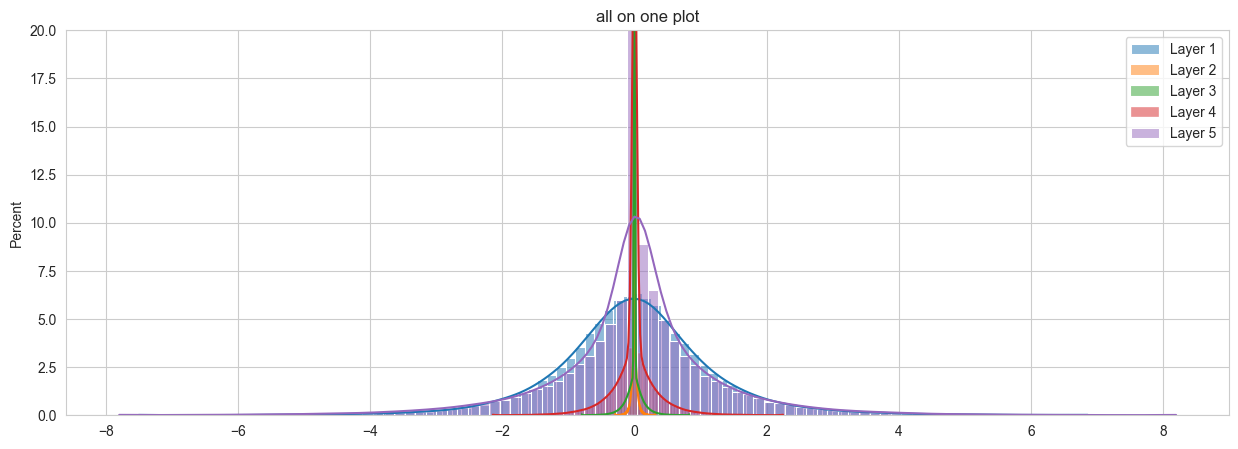
\includegraphics[width=1\textwidth]{Chapters/chapter_3_materials_methods/figures/histograms for normlization - custom cnn}
    \caption{Weight histograms of a custom CNN trained on SVHN. By focusing on the range of values, we see that the layers have different dynamic ranges, making normalization beneficial.}
    \label{fig:custom_cnn_weight_histograms}
\end{figure}

\begin{figure}[H]
    \centering
    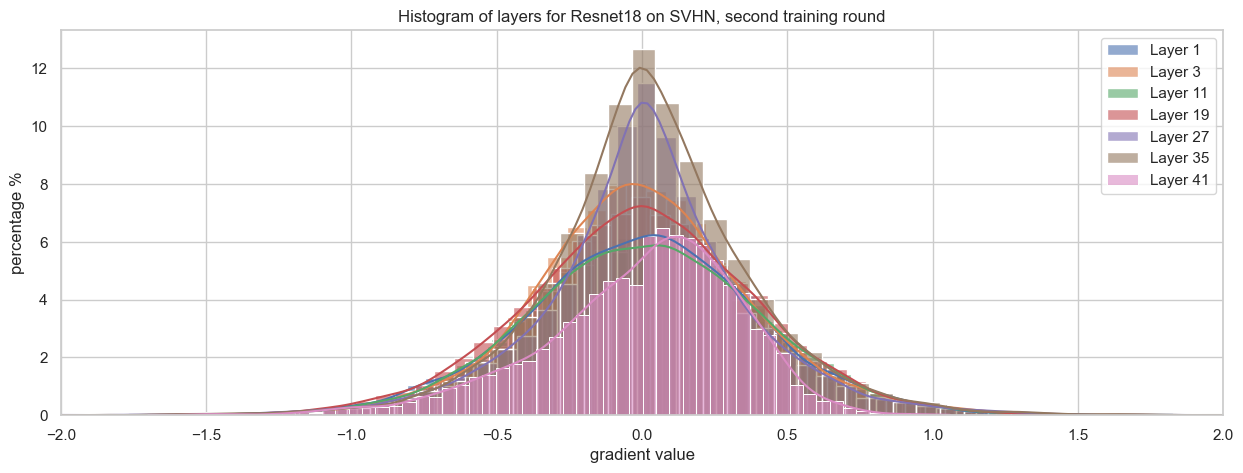
\includegraphics[width=1\textwidth]{Chapters/chapter_3_materials_methods/figures/histograms for normlization - Resnet18}
    \caption{Weight histograms of a ResNet-18 trained on SVHN. By focusing on the range of values, we see that the layers have similar dynamic ranges, making normalization unnecessary.}
    \label{fig:resnet18_weight_histograms}
\end{figure}

\subsection{Outlier Handling}
We use SGD optimizer which means our gradients are directly proportional to the change in the final loss function. This means that very large gradients have as large an impact on the loss function, and thus the training process. However, these large gradients are often treated as outliers and not reconstructed well by our WZ quantizer. As we saw in Section~3.3, the quantizer focuses on regions with high density. One could argue that the quantizer is minimizing the reconstruction loss, and thus it is doing the best job possible, but considering the very few number of outliers, we could add an additional mechanism to handle them separately and improve the overall reconstruction quality without increasing the bit rate too much.

We propose making a separate gradient vector which only includes the outliers. It is important to not remove the outliers from the original gradient vector as they will be needed to find the positions of the outliers during reconstruction. We found that values 30\% beyond the 99th percentile mark are usually not reconstructed well, but are also very few in number, around 12k for ResNet-18 on SVHN relative to more than 11 million gradient values (less than 0.1\%).

The original gradient vector is quantized normally using our WZ quantizer. For the separated values, there will be a gap between the negative and positive values caused by removing the normal values. We will remove this gap by shifting the outliers towards zero, and then we will treat them as a separate layer of the model, normalizing them and quantizing them using our WZ quantizer. Later when reconstructing, we will reverse this gap removal. This does mean that we need to send the parameters relating to the normalization and size of the gap, which is usually only a few numbers. It is important to also send the sign of the outliers, as the majority will be mapped to zero and lose their sign. The overhead for these signs is also minimal, usually less than a KB, which is negligible compared to the size of the gradients which is in the MBs.

The hard part is sending over the position of the outlier in the gradient vector that has been quantized. Sending their index is inefficient, as these indexes usually have a high bit rate as they are big numbers due to the large size of the gradient vector. Instead we modify the bin vector which was made by quantizing the original gradient vector, with the outliers intact. We set the bins which correspond to the outliers to number of bins + 1. For this to work with the rest of the pipeline, we also need to modify the prior used by rANS (explained in the next section) to have an extra row of zeros for this new (bins\_count+1)th bin. For the outlier position this value is set to a non-zero value. This does not seem to really affect the compression rate of the bin vector when using rANS.

In Figure~\ref{fig:outlier_effect_on_convergence}, we can see the effect of outlier handling on the convergence speed of the ResNet-18 on SVHN. We can see that the outlier handling significantly improves the convergence speed and makes it comparable to the unquantized model.

\begin{figure}[H]
    \centering
    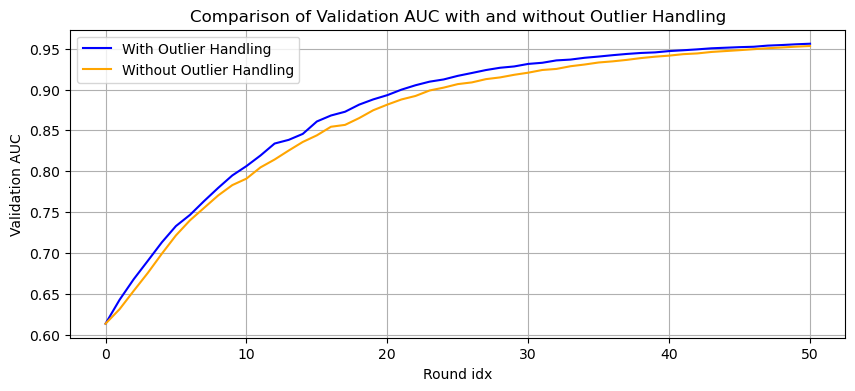
\includegraphics[width=1\textwidth]{Chapters/chapter_3_materials_methods/figures/outlierhandling effect}
    \caption{Effect of outliers on reconstruction quality. We can see that the outliers are not reconstructed well, and thus have a high reconstruction error.}
    \label{fig:outlier_effect_on_convergence}
\end{figure}
